% =============================================================================
% PARTE I: FUNDAMENTOS FÍSICOS, CINÉTICA Y QUÍMICA DEL FUEGO
% =============================================================================

% --- SLIDE 3: FUEGO VS INCENDIO ---
\begin{frame}{Fuego frente a Incendio}
  \begin{columns}[T]
    \begin{column}{0.48\textwidth}
      \begin{block}{\textbf{Fuego}}
        \small
        $\bullet$ Reacción fisicoquímica de óxido-reducción fuertemente exotérmica.\\
        $\bullet$ Emisión de luz, calor y humos.\\
        $\bullet$ \textbf{Condición operativa:} Parámetros espaciales, temporales y de combustible están gobernados por el ser humano.
      \end{block}
      \vspace{0.2cm}
      \centering
      \resizebox{0.9\columnwidth}{!}{%
        \begin{tikzpicture}
          \node[draw=successgreen!80!black, fill=successgreen!10, rounded corners=4pt, line width=1.2pt, inner sep=6pt, text width=5cm, align=center] {
            \textbf{Energía Aprovechable}\\[2pt]
            \scriptsize Hornos $\cdot$ Calderas
          };
        \end{tikzpicture}
      }
    \end{column}

    \begin{column}{0.48\textwidth}
      \begin{alertblock}{\textbf{Incendio (Siniestro Descontrolado)}}
        \small
        $\bullet$ Fuego que escapa a las barreras de contención.\\
        $\bullet$ Se propaga \textbf{sin control en el tiempo ni en el espacio}.\\
        $\bullet$ Destrucción de estructuras, ruina de activos y riesgo severo para la integridad de los operarios.
      \end{alertblock}
      \vspace{0.2cm}
      \centering
      \resizebox{0.9\columnwidth}{!}{%
        \begin{tikzpicture}
          \node[draw=firered!80!black, fill=firered!10, rounded corners=4pt, line width=1.2pt, inner sep=6pt, text width=5cm, align=center] {
            \textbf{Siniestro Destructivo}\\[2pt]
            \scriptsize Colapso edilicio $\cdot$ Gases letales $\cdot$ Pérdidas humanas
          };
        \end{tikzpicture}
      }
    \end{column}
  \end{columns}
\end{frame}

% --- SLIDE 4: TRIÁNGULO DEL FUEGO ---
\begin{frame}{Modelo Clásico: El Triángulo del Fuego}
  \begin{columns}[c]
    \begin{column}{0.48\textwidth}
      \small
      Para que exista combustión deben converger tres elementos simultáneos:
      \begin{enumerate}
        \scriptsize
        \item \textbf{Combustible:} Sustancia reductora susceptible de oxidarse (sólido, líquido o gas).
        \item \textbf{Comburente:} Agente oxidante ($O_2$ del aire; requiere concentración $\ge 14\text{--}15\%$).
        \item \textbf{Calor / Energía de activación:} Aporte térmico para alcanzar la temperatura de ignición.
      \end{enumerate}
      \vspace{0.15cm}
      \begin{alertblock}{\textbf{Mecanismos Clásicos de Extinción}}
        \scriptsize
        $\bullet$ \textbf{Desalimentación:} Supresión física del combustible.\\
        $\bullet$ \textbf{Sofocación:} Aislamiento o desplazamiento del $O_2$.\\
        $\bullet$ \textbf{Enfriamiento:} Disipación de calor por debajo del punto de ignición.
      \end{alertblock}
    \end{column}

    \begin{column}{0.50\textwidth}
      \centering
      \resizebox{0.95\columnwidth}{!}{%
        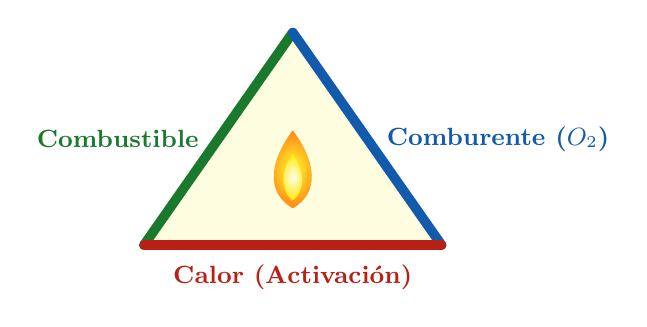
\begin{tikzpicture}[scale=0.9, line join=round, line cap=round]
          \definecolor{cCalor}{RGB}{205, 35, 25}
          \definecolor{cComb}{RGB}{30, 135, 50}
          \definecolor{cOx}{RGB}{20, 100, 190}

          \coordinate (A) at (0, 2.0);
          \coordinate (B) at (-2.1, -1.0);
          \coordinate (C) at (2.1, -1.0);

          \fill[yellow!12] (A) -- (B) -- (C) -- cycle;

          \draw[cComb!90!black, line width=3.5pt] (A) -- node[left=2pt, font=\bfseries\small, cComb!90!black]{Combustible} (B);
          \draw[cOx!90!black, line width=3.5pt] (A) -- node[right=2pt, font=\bfseries\small, cOx!90!black]{Comburente ($O_2$)} (C);
          \draw[cCalor!90!black, line width=3.5pt] (B) -- node[below=2pt, font=\bfseries\small, cCalor!90!black]{Calor (Activación)} (C);

          \begin{scope}[shift={(0, -0.15)}, scale=0.55]
            \shade[inner color=yellow!90!white, outer color=orange!95!red, opacity=0.9]
              (0,-0.6) .. controls (-0.7,-0.2) and (-0.6,0.6) .. (0,1.4)
                       .. controls (0.6,0.6) and (0.7,-0.2) .. (0,-0.6);
            \shade[inner color=white, outer color=yellow!85!orange, opacity=0.95]
              (0,-0.4) .. controls (-0.35,-0.1) and (-0.3,0.3) .. (0,0.8)
                       .. controls (0.3,0.3) and (0.35,-0.1) .. (0,-0.4);
          \end{scope}
        \end{tikzpicture}
      }
    \end{column}
  \end{columns}
\end{frame}

% --- SLIDE 5: TETRAEDRO DEL FUEGO ---
\begin{frame}{Evolución Teórica: El Tetraedro del Fuego}
  \begin{columns}[c]
    \begin{column}{0.48\textwidth}
      \small
      En la combustión viva con llama no basta con la presencia simultánea de combustible, oxígeno y calor.
      \begin{block}{\textbf{El Cuarto Elemento: Reacción en Cadena}}
        \scriptsize
        $\bullet$ La combustión se autosostiene mediante radicales libres intermedios altamente inestables ($H^\bullet, OH^\bullet, O^{\bullet\bullet}$).\\
        $\bullet$ Los choques moleculares en fase gaseosa generan una cascada autosostenida de propagación exotérmica.
      \end{block}
      \vspace{0.15cm}
      \begin{alertblock}{\textbf{Inhibición Química}}
        \scriptsize
        Extintores como polvos secos (PQS) y gases limpios capturan químicamente estos radicales libres, suprimiendo la llama al instante sin necesidad de enfriamiento masivo ni sofocación.
      \end{alertblock}
    \end{column}

    \begin{column}{0.50\textwidth}
      \centering
      \resizebox{0.95\columnwidth}{!}{%
        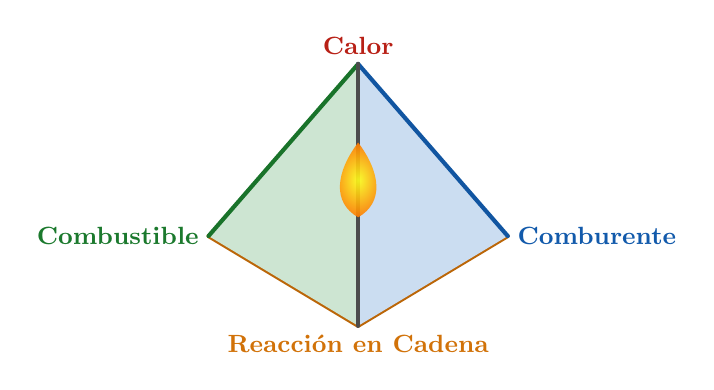
\begin{tikzpicture}[scale=0.95, line join=round, line cap=round]
          \definecolor{cCalor}{RGB}{205, 35, 25}
          \definecolor{cComb}{RGB}{30, 135, 50}
          \definecolor{cOx}{RGB}{20, 100, 190}
          \definecolor{cCad}{RGB}{220, 120, 10}

          \coordinate (T) at (0, 2.1);
          \coordinate (L) at (-2.0, -0.2);
          \coordinate (R) at (2.0, -0.2);
          \coordinate (F) at (0, -1.4);

          \fill[cCalor!16] (T) -- (L) -- (R) -- cycle;
          \draw[cCalor!60!black, line width=0.8pt, dashed] (L) -- (R);

          \fill[cCad!24] (L) -- (F) -- (R) -- cycle;
          \draw[cCad!85!black, line width=1.5pt] (L) -- (F) -- (R);

          \fill[cComb!22] (T) -- (L) -- (F) -- cycle;
          \draw[cComb!85!black, line width=1.5pt] (T) -- (L);

          \fill[cOx!22] (T) -- (F) -- (R) -- cycle;
          \draw[cOx!85!black, line width=1.5pt] (T) -- (R);
          \draw[black!70, line width=1.6pt] (T) -- (F);

          \node[above, font=\bfseries\small, cCalor!90!black] at (T) {Calor};
          \node[left, font=\bfseries\small, cComb!90!black] at (L) {Combustible};
          \node[right, font=\bfseries\small, cOx!90!black] at (R) {Comburente};
          \node[below, font=\bfseries\small, cCad!95!black] at (F) {Reacción en Cadena};

          \begin{scope}[shift={(0, 0.35)}, scale=0.5]
            \shade[inner color=yellow!90!white, outer color=orange!95!red, opacity=0.9]
              (0,-0.6) .. controls (-0.7,-0.2) and (-0.6,0.6) .. (0,1.4)
                       .. controls (0.6,0.6) and (0.7,-0.2) .. (0,-0.6);
          \end{scope}
        \end{tikzpicture}
      }
    \end{column}
  \end{columns}
\end{frame}

% --- SLIDE 6: CURVA TEMPORAL DEL INCENDIO ---
\begin{frame}{Curva Temporal de Desarrollo del Incendio y \textit{Flashover}}
  \begin{columns}[c]
    \begin{column}{0.48\textwidth}
      \small
      Dinámica del incendio en recintos confinados:
      \begin{enumerate}
        \scriptsize
        \item \textbf{Fase Incipiente / Latente:} Calor localizado, humos visibles, combustión lenta.
        \item \textbf{Fase de Crecimiento:} Acumulación de gases calientes bajo el techo; penacho térmico activo.
        \item \textbf{Flashover (Combustión Súbita Generalizada):} Salto térmico a $\sim 600\,\Celsius$. Todos los combustibles expuestos se inflaman simultáneamente por radiación.
        \item \textbf{Fase Plenamente Desarrollada:} Fuego gobernado por la ventilación disponible.
        \item \textbf{Decaimiento:} Agotamiento de combustible o extinción activa.
      \end{enumerate}
    \end{column}

    \begin{column}{0.50\textwidth}
      \centering
      \resizebox{0.95\columnwidth}{!}{%
        \begin{tikzpicture}[xscale=0.7, yscale=0.5, line cap=round, line join=round]
          \draw[->, >=stealth, line width=1pt] (0,0) -- (8.5,0) node[right, font=\scriptsize] {Tiempo};
          \draw[->, >=stealth, line width=1pt] (0,0) -- (0,7.2) node[above, font=\scriptsize] {Temperatura};

          % Curva
          \draw[line width=1.8pt, firered] (0,0.4) -- (1.5,0.7) 
                .. controls (3,1.2) and (3.8,2.2) .. (4.2,5.5) 
                -- (6.0,5.8) 
                .. controls (7.0,4.0) .. (8.0,1.5);

          % Puntos y zonas
          \draw[dashed, grayborder!80!black] (4.2,0) -- (4.2,5.5);
          \node[circle, fill=fireorange, inner sep=2pt] at (4.2,5.5) {};
          \node[above, font=\bfseries\scriptsize, firered] at (4.2,5.7) {Flashover};

          \node[font=\tiny, align=center] at (1.5, -0.6) {1. Inicial};
          \node[font=\tiny, align=center] at (3.2, -0.6) {2. Crecim.};
          \node[font=\tiny, align=center] at (5.2, -0.6) {4. Total};
          \node[font=\tiny, align=center] at (7.2, -0.6) {5. Decaim.};

          \draw[<->, >=stealth, line width=0.8pt, successgreen!80!black] (0,6.5) -- (3.8,6.5) node[midway, above, font=\scriptsize\bfseries] {Ventana de Extinción y Escape};
        \end{tikzpicture}
      }
    \end{column}
  \end{columns}
\end{frame}

% --- SLIDE 7: ESCALA DE VELOCIDADES DE COMBUSTIÓN ---
\begin{frame}{Regímenes de Combustión}
  \small
  La combustión se clasifica rigurosamente según la velocidad lineal de avance del frente reactivo:

  \vspace{0.3cm}
  \centering
  \resizebox{0.95\textwidth}{!}{%
    \begin{tikzpicture}[xscale=1.2, line cap=round, line join=round]
      % Eje horizontal
      \draw[->, >=stealth, line width=1.5pt, darkcharcoal] (0,0) -- (10.5,0) node[right, font=\small\bfseries] {Velocidad};

      % Marcas
      \draw[line width=1.2pt] (1.0, 0.2) -- (1.0, -0.2) node[below=4pt, font=\scriptsize, align=center] {Oxidación\\Lenta};
      \draw[line width=1.2pt] (3.5, 0.2) -- (3.5, -0.2) node[below=4pt, font=\scriptsize, align=center] {Combustión\\Simple};
      \draw[line width=1.5pt, fireorange] (6.0, 0.3) -- (6.0, -0.3) node[below=4pt, font=\scriptsize\bfseries, fireorange, align=center] {Deflagración\\($1\text{--}333\,\mathrm{m/s}$)};
      \draw[line width=2.0pt, firered] (8.5, 0.4) -- (8.5, -0.4) node[below=4pt, font=\scriptsize\bfseries, firered, align=center] {Detonación\\($> 333\,\mathrm{m/s}$)};

      \draw[dashed, line width=1pt, firered] (7.2, 1.8) -- (7.2, -0.8) node[below, font=\fontsize{4}{5}\selectfont, firered] {Barrera del Sonido};

      % Regiones superiores
      \node[fill=successgreen!15, rounded corners=3pt, inner sep=4pt, font=\tiny, align=center] at (2.2, 1.2) {Sin llamas vivas\\(Corrosión, carbón)};
      \node[fill=amberyellow!20, rounded corners=3pt, inner sep=4pt, font=\tiny, align=center] at (4.5, 1.2) {Frente subsónico\\$< 1\,\mathrm{m/s}$ (Madera, papel)};
      \node[fill=fireorange!20, rounded corners=3pt, inner sep=4pt, font=\tiny, align=center] at (6.4, 1.2) {Presiones $1\text{--}10\,\mathrm{atm}$\\$1700\text{--}1800\,\Celsius$};
      \node[fill=firered!20, rounded corners=3pt, inner sep=4pt, font=\tiny, align=center] at (9.0, 1.2) {Onda de choque supersónica\\Presiones $> 100\,\mathrm{atm}$};
    \end{tikzpicture}
  }
\end{frame}

% --- SLIDE 8: DEFLAGRACIÓN VS DETONACIÓN ---
\begin{frame}{Física de la Deflagración y la Detonación}
  \begin{columns}[T]
    \begin{column}{0.48\textwidth}
      \begin{block}{\textbf{Deflagración (Subsónica)}}
        \small
        $\bullet$ Velocidad de llama entre $1\m/\mathrm{s}$ y $333\m/\mathrm{s}$.\\
        $\bullet$ La propagación térmica se realiza por conducción y difusión de calor hacia la mezcla no quemada.\\
        $\bullet$ \textbf{Sobrepresión:} $1$ a $10$ veces la presión inicial del recinto.\\
        $\bullet$ \textbf{Temperatura:} $1700\,\Celsius$ a $1800\,\Celsius$.\\
        $\bullet$ Genera bolas de fuego (\textit{flashes}) y graves quemaduras cutáneas por radiación.
      \end{block}
    \end{column}

    \begin{column}{0.48\textwidth}
      \begin{alertblock}{\textbf{Detonación (Supersónica)}}
        \small
        $\bullet$ Velocidad superior a la del sonido ($> 333\m/\mathrm{s}$, alcanzando miles de $\m/\mathrm{s}$).\\
        $\bullet$ La combustión está acoplada a una onda de choque mecánica que autocomprime los reactivos adiabáticamente.\\
        $\bullet$ \textbf{Sobrepresión:} Supera en más de $100$ veces la presión inicial.\\
        $\bullet$ \textbf{Efecto mecánico:} Destrucción física de tabiques, muros y maquinaria pesada en milisegundos.
      \end{alertblock}
    \end{column}
  \end{columns}
\end{frame}

% --- SLIDE 9: MECANISMOS DE TRANSFERENCIA DE CALOR ---
\begin{frame}{Mecanismos de Propagación Térmica del Fuego}
  \begin{columns}[c]
    \begin{column}{0.48\textwidth}
      \small
      El fuego se propaga en un edificio por tres fenómenos termodinámicos simultáneos:
      \begin{itemize}
        \scriptsize
        \item \textbf{Conducción:} Transmisión de energía cinética molecular a través de sólidos continuos (vigas de acero, cañerías metálicas que transmiten calor a recintos vecinos).
        \item \textbf{Convección:} Transporte térmico por desplazamiento de masas de fluidos y humos sobrecalentados que ascienden por flotabilidad (efecto chimenea).
        \item \textbf{Radiación:} Emisión de ondas electromagnéticas infrarrojas en línea recta sin necesidad de medio material interpuesto.
      \end{itemize}
    \end{column}

    \begin{column}{0.50\textwidth}
      \centering
      \resizebox{0.95\columnwidth}{!}{%
        \begin{tikzpicture}[scale=0.85]
          % Foco
          \node[draw=firered, fill=firered!20, circle, inner sep=6pt, font=\bfseries\scriptsize] (F) at (0,0) {Foco};

          % Conducción
          \draw[->, >=stealth, line width=1.5pt, darkcharcoal] (F) -- (3,0) node[right, font=\scriptsize\bfseries] {Conducción (Estructura)};
          % Convección
          \draw[->, >=stealth, line width=1.5pt, fireorange] (F) -- (0,2.5) node[above, font=\scriptsize\bfseries] {Convección (Gases calientes)};
          % Radiación
          \draw[->, >=stealth, line width=1.5pt, firered] (F) -- (2.2,2.0) node[above right, font=\scriptsize\bfseries] {Radiación ($\sigma T^4$)};
          \draw[->, >=stealth, line width=1.5pt, firered] (F) -- (-2.2,2.0) node[above left, font=\scriptsize\bfseries] {Radiación};
        \end{tikzpicture}
      }
    \end{column}
  \end{columns}
\end{frame}

% --- SLIDE 10: LÍMITES DE INFLAMABILIDAD ---
\begin{frame}{Termodinámica: Límites de Inflamabilidad en Aire}
  \small
  Para que una mezcla gas/aire se inflame, la concentración de combustible debe ubicarse estrictamente en su rango reactivo:

  \vspace{0.3cm}
  \centering
  \resizebox{0.92\textwidth}{!}{%
    \begin{tikzpicture}[xscale=1.1, line cap=round, line join=round]
      % Barra horizontal de concentración
      \draw[line width=1.2pt, darkcharcoal] (0,0) rectangle (10,1);

      % Zona Pobre
      \fill[gray!20] (0,0) rectangle (2.5,1);
      \node[font=\scriptsize\bfseries, align=center] at (1.25, 0.5) {Mezcla Pobre\\(No arde)};

      % Rango Inflamable
      \fill[firered!30] (2.5,0) rectangle (7.5,1);
      \node[font=\scriptsize\bfseries, firered!90!black, align=center] at (5.0, 0.5) {RANGO INFLAMABLE\\(Propagación de Llama)};

      % Zona Rica
      \fill[gray!20] (7.5,0) rectangle (10,1);
      \node[font=\scriptsize\bfseries, align=center] at (8.75, 0.5) {Mezcla Rica\\(Falta $O_2$)};

      % Límites
      \draw[line width=2pt, firered] (2.5,-0.3) -- (2.5,1.3) node[above, font=\scriptsize\bfseries] {LII (Límite Inferior)};
      \draw[line width=2pt, firered] (7.5,-0.3) -- (7.5,1.3) node[above, font=\scriptsize\bfseries] {LSI (Límite Superior)};

      % Flecha inferior de temperatura
      \node[below, font=\tiny, align=center] at (5.0, -0.5) {El incremento de la temperatura ambiental incrementa la presión de vapor y \textbf{ensancha el rango reactivo}.};
    \end{tikzpicture}
  }
\end{frame}

% --- SLIDE 11: TEMPERATURAS CRÍTICAS ---
\begin{frame}{Temperaturas Críticas de Inflamación de Sustancias}
  \begin{columns}[c]
    \begin{column}{0.52\textwidth}
      \begin{block}{\textbf{1. Inflamación }}
        \scriptsize Temperatura mínima donde los vapores forman mezcla inflamable y destellan ante llama externa (se apagan al retirar la fuente).
      \end{block}
      \begin{block}{\textbf{2. Punto de Fuego }}
        \scriptsize Temperatura superior donde la evaporación sostiene la combustión continua con llama por $\ge 5\,\mathrm{s}$.
      \end{block}
      \begin{alertblock}{\textbf{3. Temperatura de Autoignición}}
        \scriptsize Umbral térmico donde la energía interna activa la combustión espontánea y autosostenida \textbf{sin llama ni chispa piloto}.
      \end{alertblock}
    \end{column}

    \begin{column}{0.44\textwidth}
      \centering
      \resizebox{0.75\columnwidth}{!}{%
        \begin{tikzpicture}[yscale=0.7]
          \draw[line width=2pt, ->, >=stealth, darkcharcoal] (0,0) -- (0,5.2) node[above, font=\scriptsize\bfseries] {Temperatura ($\Celsius$)};
          \draw[fill=firered!20, draw=firered, line width=1.2pt] (-1.5,3.8) rectangle (1.5,4.6) node[midway, font=\tiny\bfseries, align=center] {Autoignición\\(Espontáneo)};
          \draw[fill=fireorange!20, draw=fireorange, line width=1.2pt] (-1.5,2.1) rectangle (1.5,2.9) node[midway, font=\tiny\bfseries, align=center] {Punto de Fuego\\(Sostenido)};
          \draw[fill=amberyellow!20, draw=amberyellow, line width=1.2pt] (-1.5,0.4) rectangle (1.5,1.2) node[midway, font=\tiny\bfseries, align=center] {Flash Point\\(Destello)};
        \end{tikzpicture}
      }
    \end{column}
  \end{columns}
\end{frame}

% --- SLIDE 12: SIMBOLOGÍA NORMALIZADA DE CLASES DE FUEGO ---
\begin{frame}{Clasificación Normalizada de Fuegos (IRAM 3517 / NFPA 10)}
  \small
  Identificación visual de las cinco clases de fuego según combustible y mecanismo de extinción:

  \vspace{0.2cm}
  \centering
  \resizebox{0.98\textwidth}{!}{%
    \begin{tikzpicture}[xscale=2.2, line cap=round, line join=round]
      % Clase A
      \node[regular polygon, regular polygon sides=3, draw=successgreen!90!black, fill=successgreen!20, line width=1.5pt, inner sep=4pt] (A) at (0,0) {\bfseries\large A};
      \node[below=20pt, font=\tiny, align=center] at (A) {\textbf{Sólidos Orgánicos}\\Madera, papel, telas\\Residuos con brasas};

      % Clase B
      \node[regular polygon, regular polygon sides=4, draw=firered!90!black, fill=firered!20, line width=1.5pt, inner sep=5pt] (B) at (1.2,0) {\bfseries\large B};
      \node[below=20pt, font=\tiny, align=center] at (B) {\textbf{Líquidos y Gases}\\Naftas, solventes, aceites\\Combustión superficial};

      % Clase C
      \node[circle, draw=utnblue!90!black, fill=utnblue!20, line width=1.5pt, inner sep=4pt] (C) at (2.4,0) {\bfseries\large C};
      \node[below=20pt, font=\tiny, align=center] at (C) {\textbf{Equipos Eléctricos}\\Tableros energizados\\Riesgo de electrocución};

      % Clase D
      \node[star, star points=5, star point ratio=2.2, draw=amberyellow!90!black, fill=amberyellow!25, line width=1.5pt, inner sep=2pt] (D) at (3.6,0) {\bfseries\large D};
      \node[below=20pt, font=\tiny, align=center] at (D) {\textbf{Metales Reactivos}\\Magnesio, sodio, titanio\\Polvos especiales};

      % Clase K
      \node[regular polygon, regular polygon sides=6, draw=darkcharcoal, fill=darkcharcoal!15, line width=1.5pt, inner sep=4pt] (K) at (4.8,0) {\bfseries\large K};
      \node[below=20pt, font=\tiny, align=center] at (K) {\textbf{Grasas y Aceites}\\Cocinas industriales\\Saponificación alcalina};
    \end{tikzpicture}
  }
\end{frame}

% --- SLIDE 13: FUEGOS CLASE A Y B ---
\begin{frame}{Dinámica de Combustión: Fuegos Clase A frente a Clase B}
  \begin{columns}[T]
    \begin{column}{0.48\textwidth}
      \begin{block}{\textbf{Fuegos Clase A: En Profundidad}}
        \small
        $\bullet$ Combustión en masa de sólidos porosos con formación de \textbf{brasas carbonosas} e incandescencia interna.\\
        $\bullet$ La extinción exige penetración y absorción de calor mediante agua con alto calor latente ($2260\,\mathrm{kJ/kg}$).
      \end{block}
      \vspace{0.2cm}
      \centering
      \resizebox{0.8\columnwidth}{!}{%
        \begin{tikzpicture}
          \draw[fill=darkcharcoal!30, line width=1pt] (0,0) rectangle (3,1.2);
          \fill[firered!80] (0.8,0.2) circle (0.3);
          \fill[firered!80] (2.2,0.4) circle (0.25);
          \node[font=\tiny\bfseries, white] at (1.5,0.7) {Brasas Internas};
        \end{tikzpicture}
      }
    \end{column}

    \begin{column}{0.48\textwidth}
      \begin{block}{\textbf{Fuegos Clase B: Superficiales}}
        \small
        $\bullet$ El líquido en sí no arde; arden exclusivamente los vapores desprendidos en la interfase líquido-aire.\\
        $\bullet$ Extinción por rotura de interfase: sellado con película acuosa (espumas AFFF) o inhibición química (PQS).
      \end{block}
      \vspace{0.2cm}
      \centering
      \resizebox{0.8\columnwidth}{!}{%
        \begin{tikzpicture}
          \draw[fill=utncyan!20, line width=1pt] (0,0) rectangle (3,0.8);
          \draw[firered, line width=2pt] (0,0.8) -- (3,0.8);
          \node[above, font=\tiny\bfseries, firered] at (1.5,0.9) {Llamas en Interfase Gaseosa};
          \node[font=\tiny, darkcharcoal] at (1.5,0.4) {Líquido Inflamable};
        \end{tikzpicture}
      }
    \end{column}
  \end{columns}
\end{frame}

% --- SLIDE 14: FUEGOS CLASE C ---
\begin{frame}{Fuegos Clase C: El Riesgo Dieléctrico en Electrónica}
  \begin{columns}[c]
    \begin{column}{0.48\textwidth}
      \small
      La particularidad de la Clase C radica en la presencia de potencial eléctrico:
      \begin{itemize}
        \scriptsize
        \item \textbf{Peligro Primario:} Choque eléctrico letal a través del chorro extintor si se emplea un agente conductor (e.g. agua común o espumas salinas).
        \item \textbf{Agentes Homologados:} Rigurosamente no conductores ($CO_2$, gases limpios FK-5-1-12, polvos químicos secos dieléctricos).
        \item \textbf{Reclasificación Operativa:} Una vez desenergizado el seccionador principal con confirmación de tensión nula, el fuego se combate como Clase A o B según el aislamiento que continúe ardiendo.
      \end{itemize}
    \end{column}

    \begin{column}{0.50\textwidth}
      \centering
      \resizebox{0.85\columnwidth}{!}{%
        \begin{tikzpicture}
          \node[draw=firered, fill=firered!10, rounded corners=6pt, line width=1.5pt, inner sep=8pt, align=center] {
            \Large\textbf{\textcolor{firered}{RIESGO ELÉCTRICO}}\\[4pt]
            \scriptsize\textbf{PROHIBIDO EL USO DE AGUA}\\
            \scriptsize Choque eléctrico y arco secundario\\
            \scriptsize Utilizar exclusivamente $CO_2$ o Gas Limpio
          };
        \end{tikzpicture}
      }
    \end{column}
  \end{columns}
\end{frame}

% --- SLIDE 15: FUEGOS CLASE D Y K ---
\begin{frame}{Fuegos Especiales: Clase D (Metales) y Clase K (Grasas)}
  \begin{columns}[T]
    \begin{column}{0.48\textwidth}
      \begin{block}{\textbf{Clase D: Metales Combustibles}}
        \scriptsize
        $\bullet$ \textbf{Materiales:} Magnesio ($Mg$), Titanio ($Ti$), Sodio ($Na$), Potasio ($K$).\\
        $\bullet$ \textbf{Reacción violenta con agua:}
        \begin{equation*}
          \mathrm{Mg + H_2O \rightarrow MgO + H_2 \uparrow \quad (\text{Explosión})}
        \end{equation*}
        $\bullet$ \textbf{Agente extintor:} Polvos secos de sales fundentes (cloruro de sodio / grafito) que forman una costra impermeable aislante.
      \end{block}
    \end{column}

    \begin{column}{0.48\textwidth}
      \begin{block}{\textbf{Clase K: Aceites de Cocción}}
        \scriptsize
        $\bullet$ \textbf{Termodinámica:} Elevada capacidad calórica; arden a $>300\,\Celsius$ y retienen calor por prolongado tiempo.\\
        $\bullet$ \textbf{Mecanismo de Saponificación:} Solución acuosa de sales alcalinas (acetato y citrato de potasio):
        \begin{equation*}
          \text{Ácidos Grasos} + \text{Base Alcalina} \rightarrow \text{Jabón Espeso}
        \end{equation*}
        $\bullet$ Enfría y sofoca cortando la reignición espontánea.
      \end{block}
    \end{column}
  \end{columns}
\end{frame}
